% Latex file with optics project summary.
\documentclass{beamer}

% include some packages
\usepackage{color}
\usepackage[utf8]{inputenc}
\usepackage{default}
\usepackage{hyperref}
\usepackage{dcolumn}% Align table columns on decimal point

\setbeamertemplate{caption}{\insertcaption} 

% Latex file body
\begin{document}


% slide # 1 
%%%%%%%%%%%%%%%%%%%%%%%%%%%%%%%%%%%%%%%%%%%%%%%%%%%%%%%%%%%%%%%%%%%%%%%%%%%%%%%%%%%%%%%%%%%%%%%%%%%%%%%%%%%%%%%%
\begin{frame}
\textcolor{blue}{\textbf{Idea 1:}} We filter out all photons with frequencies $f < f_{g} = \frac{w_{g}}{h}$ where $w_{g}$ is a band gap energy. These photons are not able to excite electrons and, thus,
contribute to useless energy reducing the efficiency of a solar cell.\\
\vspace{0.2cm}

\textcolor{red}{Power of incident radiation} $P_{inc}$ is 

$$ P_{inc} = \int_{f_{g}}^{f_{max}}\frac{\partial P}{\partial f}df$$

where $f_{max}$ is the spectrum optimization parameter we are lookiand $f_{max} = \infty$ if the rest of the spectrum is accounted for. 

\vspace{0.2cm}

\textcolor{red}{Power delivered to the load} is
$$ P_{L} = \phi\cdot w_g  = f_{g}\cdot \int_{f_{g}}^{f_{max}}\frac{1}{f}\frac{\partial P}{\partial f}df$$
where $\phi$ is the photon flux. \textcolor{red}{\textbf{We also assume that each photon contributes only energy $w_g$ to the electric output}}. 
%Then, solar cell efficiency is 
%$$ \eta = \frac{P_{L}}{P_{inc}} = \frac{f_{g}\cdot\int_{f_{g}}^{f_{max}}\frac{1}{f}\frac{\partial P}{\partial f}df}{\int_{f_{g}}^{f_{max}}\frac{\partial P}{\partial f}df}$$ 
\end{frame}
%%%%%%%%%%%%%%%%%%%%%%%%%%%%%%%%%%%%%%%%%%%%%%%%%%%%%%%%%%%%%%%%%%%%%%%%%%%%%%%%%%%%%%%%%%%%%%%%%%%%%%%%%%%%%%%%




% slide # 2 
%%%%%%%%%%%%%%%%%%%%%%%%%%%%%%%%%%%%%%%%%%%%%%%%%%%%%%%%%%%%%%%%%%%%%%%%%%%%%%%%%%%%%%%%%%%%%%%%%%%%%%%%%%%%%%%%
\begin{frame}

\begin{center}
\textbf{Quantities we want to maximize:}
\end{center}

\textbf{1.} Solar cell efficiency
$$ \eta = \frac{P_{L}}{P_{inc}} = \frac{f_{g}\cdot\int_{f_{g}}^{f_{max}}\frac{1}{f}\frac{\partial P}{\partial f}df}{\int_{f_{g}}^{f_{max}}\frac{\partial P}{\partial f}df}$$  
%\vspace{0.2cm}
\textbf{2.} Power delivered to the load
$$ P_{L} = \phi\cdot w_g  = f_{g}\cdot \int_{f_{g}}^{f_{max}}\frac{1}{f}\frac{\partial P}{\partial f}df$$

%\begin{center}
%\textbf{Estimation of heat losses in solar cell:}
%\end{center}
%Randomized energy which appears as heat
%$$ P_{Lost} = \phi\cdot (\epsilon - w_g)  = f_{g}\cdot \int_{f_{g}}^{f_{max}}\frac{1}{f}\frac{\partial P}{\partial f}df$$
\end{frame}
%%%%%%%%%%%%%%%%%%%%%%%%%%%%%%%%%%%%%%%%%%%%%%%%%%%%%%%%%%%%%%%%%%%%%%%%%%%%%%%%%%%%%%%%%%%%%%%%%%%%%%%%%%%%%%%%




% slide # 3
%%%%%%%%%%%%%%%%%%%%%%%%%%%%%%%%%%%%%%%%%%%%%%%%%%%%%%%%%%%%%%%%%%%%%%%%%%%%%%%%%%%%%%%%%%%%%%%%%%%%%%%%%%%%%%%%
\begin{frame}{Solar spectrum model: black body radiation, $T=5880^{0}$C.}

Black body radiation spectrum (Planck's equation):
$$ \frac{\partial P}{\partial f} = \frac{2h}{c^2}\frac{f^3}{e^{\frac{hf}{k_{B}T}}-1}$$
where $T$ is the temperature of the black body radiator
\begin{figure} [t]
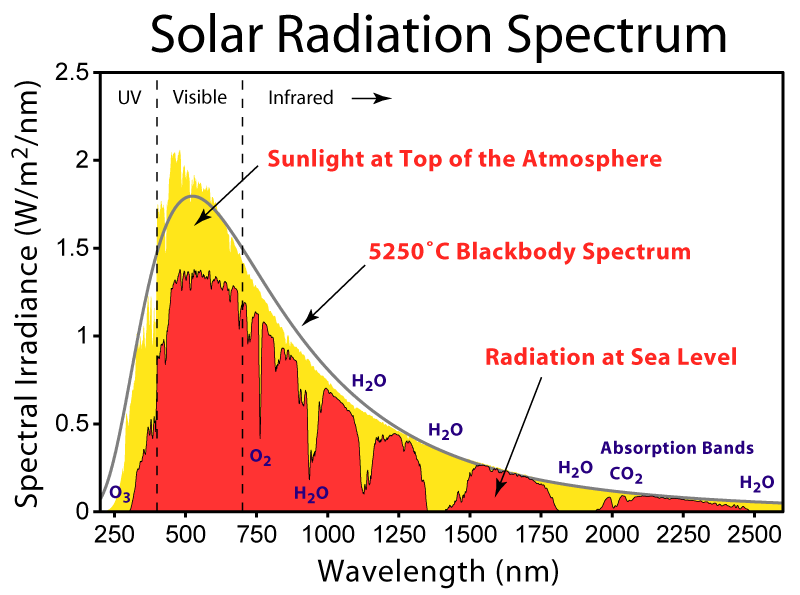
\includegraphics[width=0.75\textwidth]{figures/figure1_Solar_Spectrum.png}
%\caption{\label{fig:CT6-bands} }
\end{figure}

\end{frame}
%%%%%%%%%%%%%%%%%%%%%%%%%%%%%%%%%%%%%%%%%%%%%%%%%%%%%%%%%%%%%%%%%%%%%%%%%%%%%%%%%%%%%%%%%%%%%%%%%%%%%%%%%%%%%%%%  




% slide # 4
%%%%%%%%%%%%%%%%%%%%%%%%%%%%%%%%%%%%%%%%%%%%%%%%%%%%%%%%%%%%%%%%%%%%%%%%%%%%%%%%%%%%%%%%%%%%%%%%%%%%%%%%%%%%%%%%
\begin{frame}%{Adimensional quantities: $x = \frac{hf}{k_{B}T}$}

\textbf{1.} Solar cell (ultimate) efficiency
$$ \eta = x_{g}\frac{\int_{x_{g}}^{x_{max}}\frac{x^2}{e^x-1}dx}{\int_{x_{g}}^{x_{max}}\frac{x^3}{e^x-1}dx}$$  
%\vspace{0.2cm}
\textbf{2.} Normalized power delivered to the load

%$$ P_{L} = A f_{g}\left(\frac{k_{B}T}{h}\right)^3 \int_{x_{g}}^{x_{max}}\frac{x^2}{e^x-1}dx$$
%For solar cell made of Si, $w_{g} = 1.1$ eV and for the black body spectrum at $T = 5250^o$C, we get $x_{g} = 2.43148$.
$$ P_{L} = \frac{\int_{x_{g}}^{x_{max}}\frac{x^2}{e^x-1}dx}{\int_{x_{g}}^{\infty}\frac{x^2}{e^x-1}dx}$$

\begin{center}
\textcolor{red}{\textbf{Crossing at $W_{max} = 2.1$ eV $\Rightarrow$ region 1.1 eV $< w <$ 2.1 eV}}
\end{center}

\vspace{-0.2cm}

\begin{figure} [t]
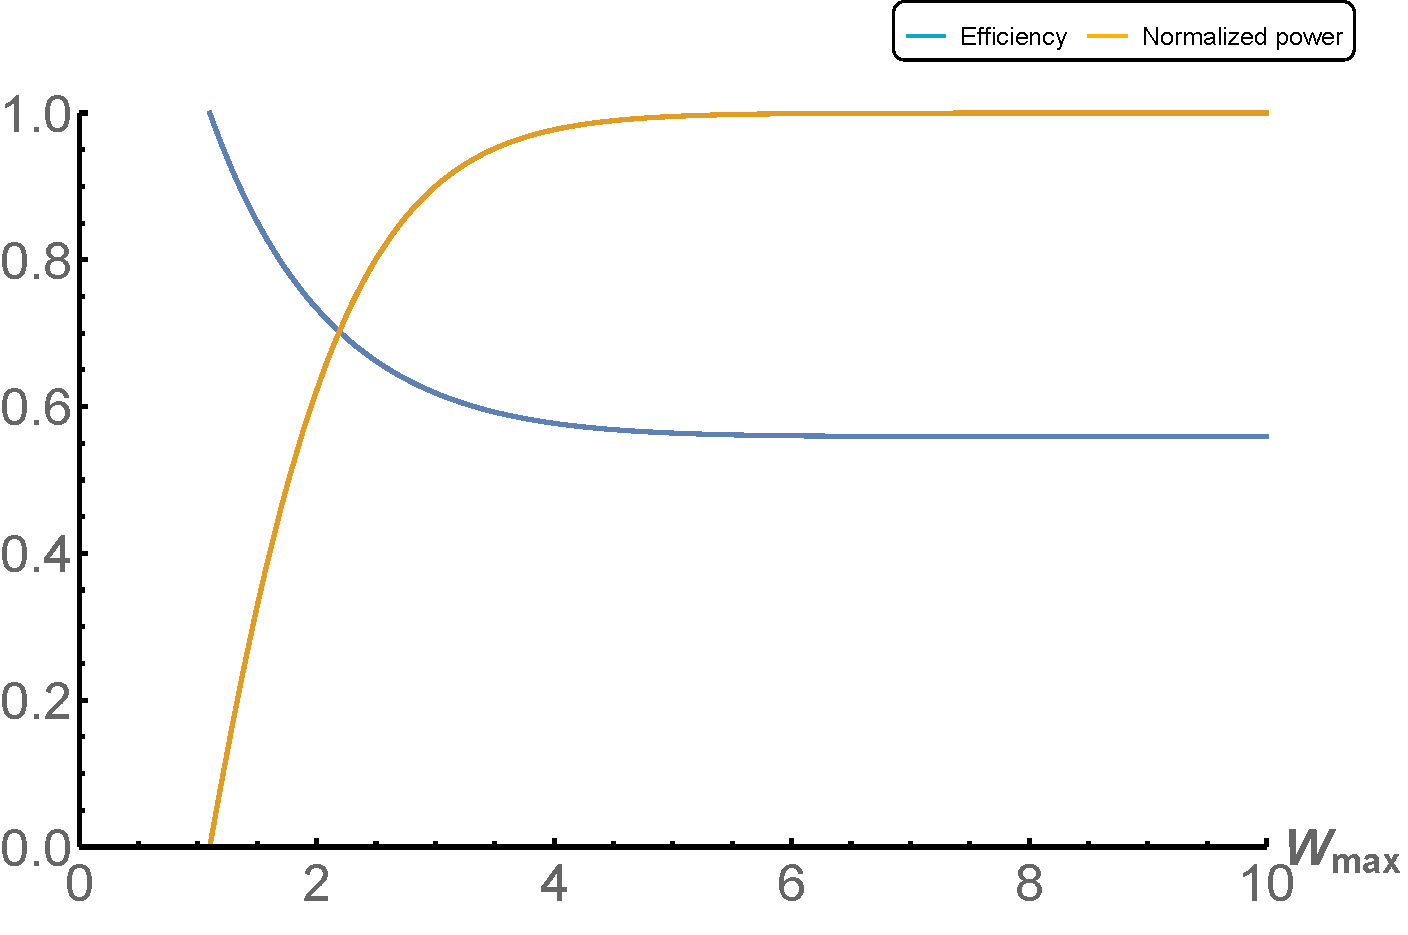
\includegraphics[width=0.6\textwidth]{figures/figure2_solar_cell_optimization.pdf}
%\caption{\label{fig:CT6-bands} }
\end{figure}

\end{frame}
%%%%%%%%%%%%%%%%%%%%%%%%%%%%%%%%%%%%%%%%%%%%%%%%%%%%%%%%%%%%%%%%%%%%%%%%%%%%%%%%%%%%%%%%%%%%%%%%%%%%%%%%%%%%%%%%




% slide # 5
%%%%%%%%%%%%%%%%%%%%%%%%%%%%%%%%%%%%%%%%%%%%%%%%%%%%%%%%%%%%%%%%%%%%%%%%%%%%%%%%%%%%%%%%%%%%%%%%%%%%%%%%%%%%%%%%
\begin{frame}{Test case: no filter for $f < f_{g}$}

Solar cell (ultimate) efficiency is 
$$ \eta (x_{g}) = x_{g}\frac{\int_{x_{g}}^{\infty}\frac{x^2}{e^x-1}dx}{\int_{0}^{\infty}\frac{x^3}{e^x-1}dx}$$  
\vspace{0.2cm}

\begin{center}
\textcolor{red}{\textbf{Maximum efficiency for band gap value $w_{g} \simeq 1.1$ eV.}}
\end{center}

\begin{figure} [t]
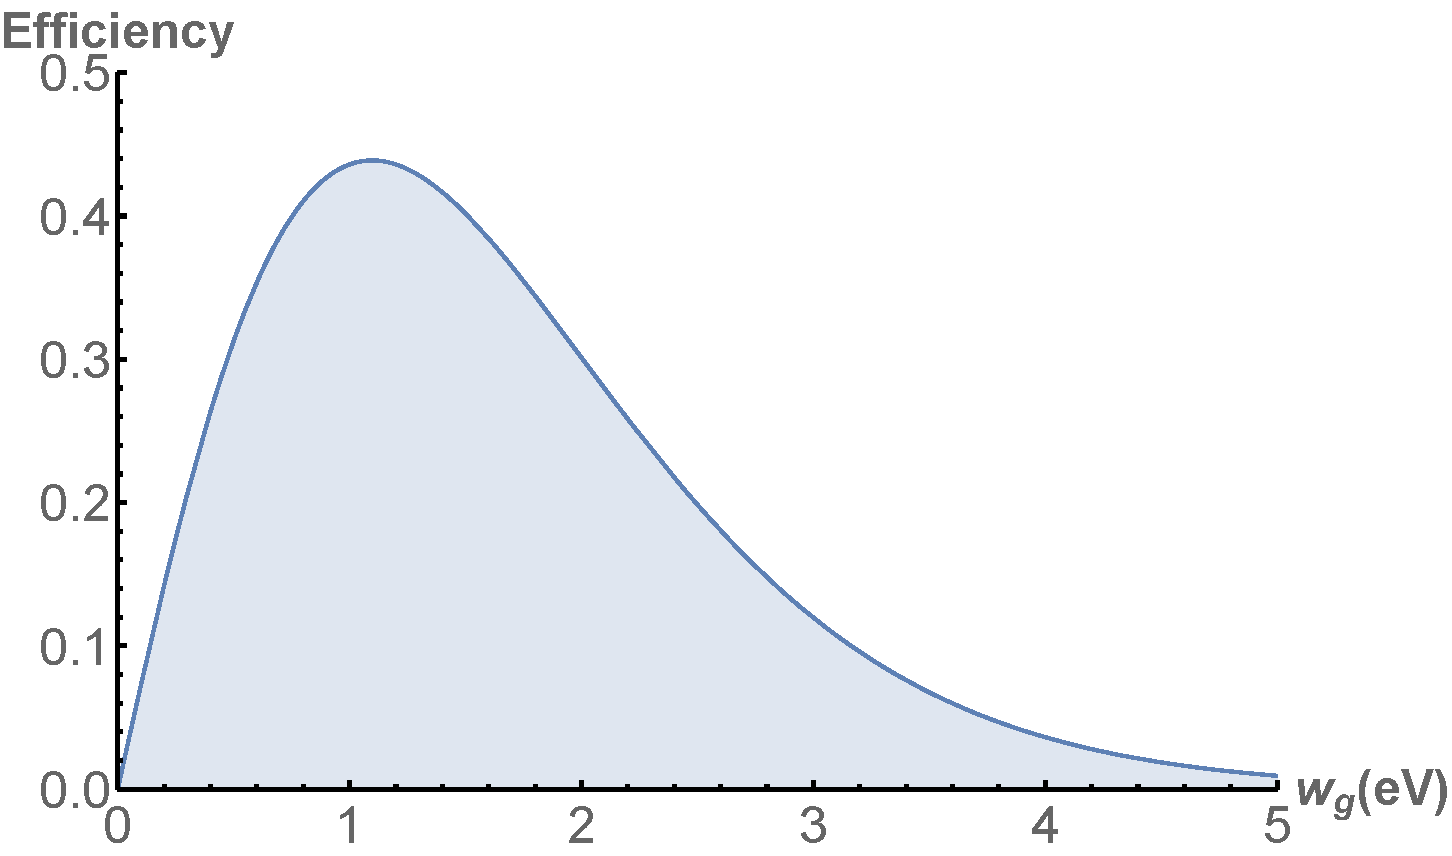
\includegraphics[width=0.6\textwidth]{figures/figure3_solar_cell_efficiency_vs_bandgap.pdf}
%\caption{\label{fig:CT6-bands} }
\end{figure}

\begin{center}
{\textbf{Matches well with the book of da Rosa.}}
\end{center}

\end{frame}
%%%%%%%%%%%%%%%%%%%%%%%%%%%%%%%%%%%%%%%%%%%%%%%%%%%%%%%%%%%%%%%%%%%%%%%%%%%%%%%%%%%%%%%%%%%%%%%%%%%%%%%%%%%%%%%%




% slide # 6
%%%%%%%%%%%%%%%%%%%%%%%%%%%%%%%%%%%%%%%%%%%%%%%%%%%%%%%%%%%%%%%%%%%%%%%%%%%%%%%%%%%%%%%%%%%%%%%%%%%%%%%%%%%%%%%%
\begin{frame}{Test case: no filter for $f < f_{g}$}

Solar cell (ultimate) efficiency for Si ($w_{g} = 1.1$ eV) is 
$$ \eta (x_{max})= x_{g}\frac{\int_{x_{g}}^{x_{max}}\frac{x^2}{e^x-1}dx}{\int_{0}^{\infty}\frac{x^3}{e^x-1}dx}$$  
\vspace{0.2cm}

\begin{center}
\textcolor{red}{\textbf{Saturation at $w_{max} \simeq 4.2$ eV.}}
\end{center}

\begin{figure} [t]
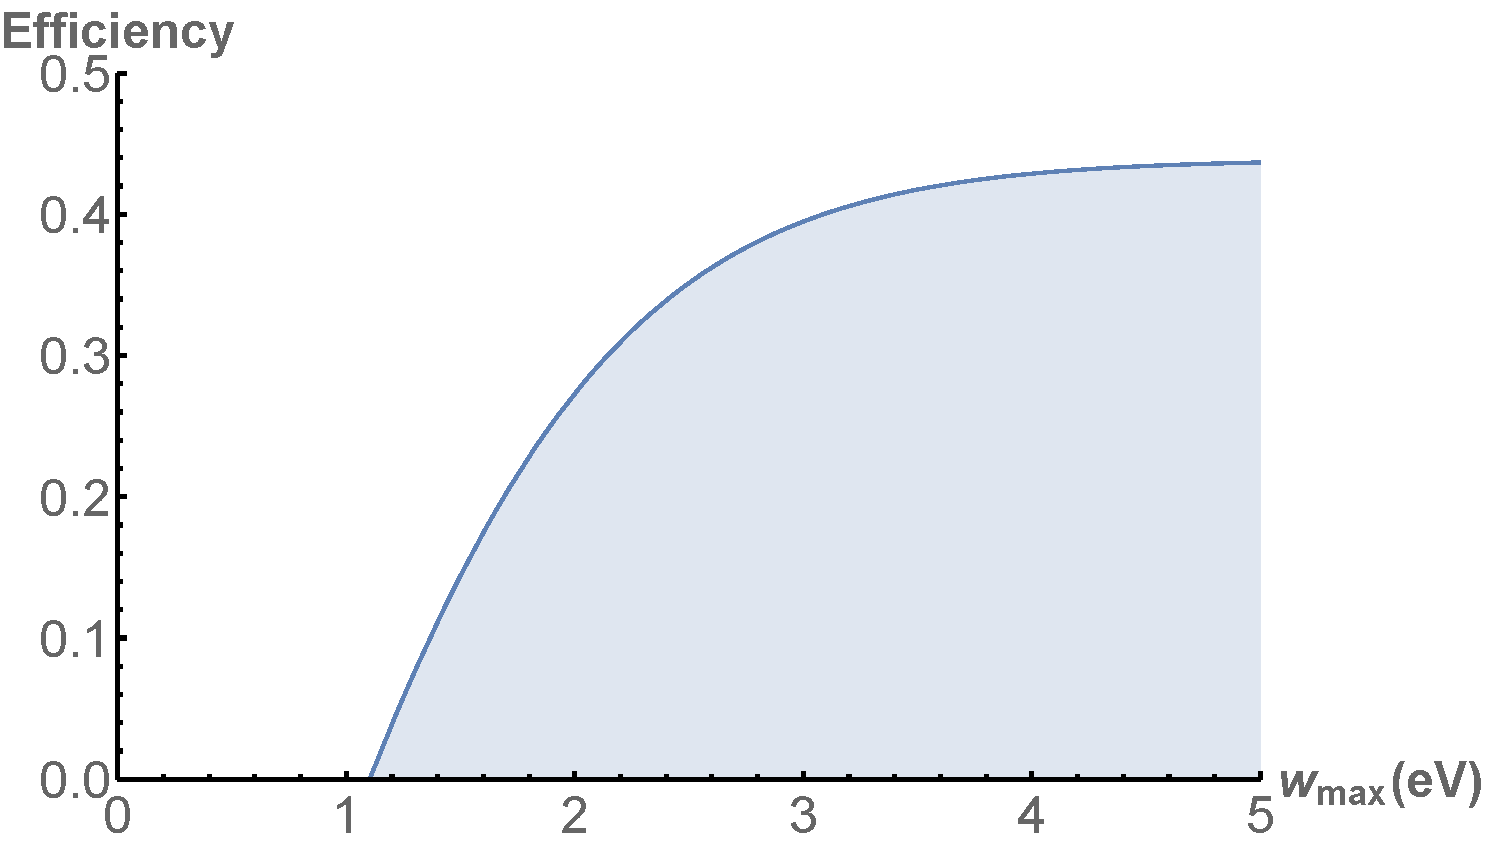
\includegraphics[width=0.6\textwidth]{figures/figure4_solar_cell_Si_efficiency_vs_wmax.pdf}
%\caption{\label{fig:CT6-bands} }
\end{figure}
\end{frame}
%%%%%%%%%%%%%%%%%%%%%%%%%%%%%%%%%%%%%%%%%%%%%%%%%%%%%%%%%%%%%%%%%%%%%%%%%%%%%%%%%%%%%%%%%%%%%%%%%%%%%%%%%%%%%%%%





% slide # 7
%%%%%%%%%%%%%%%%%%%%%%%%%%%%%%%%%%%%%%%%%%%%%%%%%%%%%%%%%%%%%%%%%%%%%%%%%%%%%%%%%%%%%%%%%%%%%%%%%%%%%%%%%%%%%%%%
\begin{frame}{Estimation of power delivered to the load}
\begin{center}
\textbf{Total radiated power (full spect.): Stephan-Boltzmann law}\\
$P_{in} = \sigma T^4 \Rightarrow$ at T = 5880$^o$K we get $P_{in}  = 6.779\cdot10^7$ W/m$^2$
\end{center}

\vspace{0.1cm}

\begin{center}
\textcolor{blue}{\textbf{Total power delivered to the load (no filter)}}\\
$ P_{L} = f_{g}\int_{f_{g}}^{\infty}\frac{1}{f}\frac{\partial P}{\partial f}df \Rightarrow$ for Si we get $P_{L}  = 2.98\cdot10^7$ W/m$^2$
\end{center}

\vspace{0.1cm}

\begin{center}
\textcolor{red}{\textbf{Total power delivered to the load (with filter)}}\\
\end{center}

\begin{figure} [t]
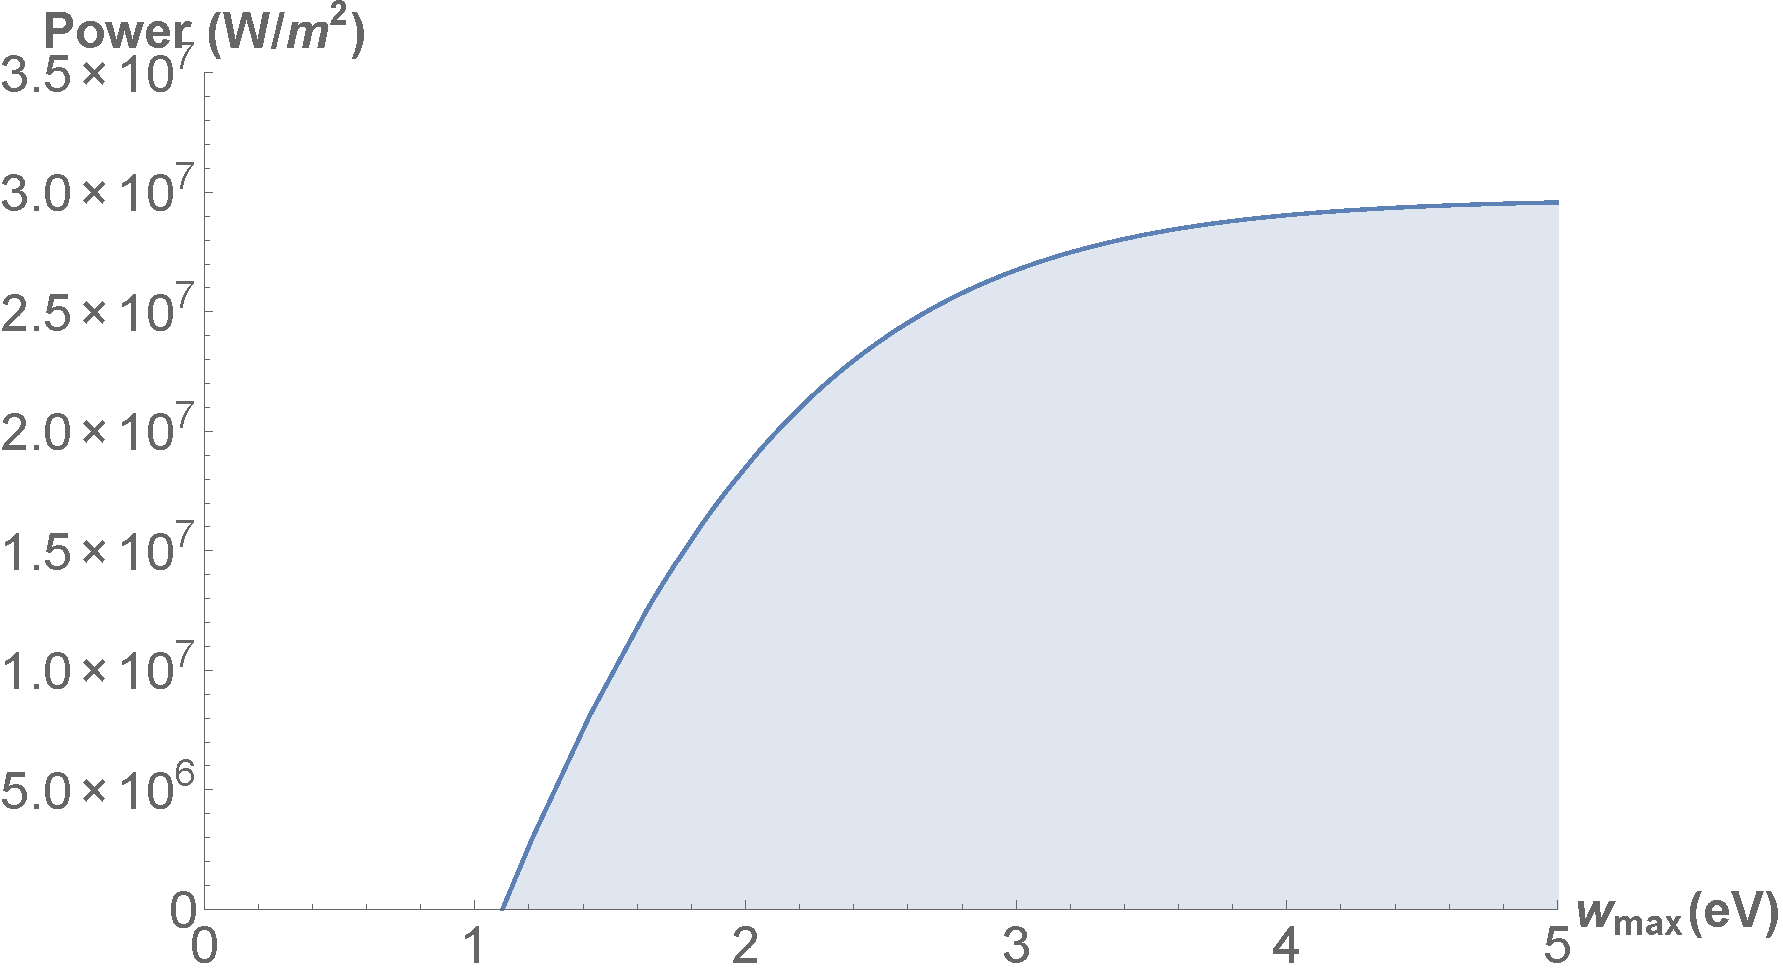
\includegraphics[width=0.6\textwidth]{figures/figure5_solar_cell_optimization_power.pdf}
%\caption{\label{fig:CT6-bands} }
\end{figure}

\vspace{-0.1cm}
\begin{center}
\textcolor{red}{\textbf{In the region $w < 2.1$ eV useful power is $P_{L} = 1.82\cdot10^7$ W/m$^2$}}
\end{center}

\end{frame}
%%%%%%%%%%%%%%%%%%%%%%%%%%%%%%%%%%%%%%%%%%%%%%%%%%%%%%%%%%%%%%%%%%%%%%%%%%%%%%%%%%%%%%%%%%%%%%%%%%%%%%%%%%%%%%%%




% slide # 8
%%%%%%%%%%%%%%%%%%%%%%%%%%%%%%%%%%%%%%%%%%%%%%%%%%%%%%%%%%%%%%%%%%%%%%%%%%%%%%%%%%%%%%%%%%%%%%%%%%%%%%%%%%%%%%%%
\begin{frame}{Power of incident light in space near Earth}

\begin{center}
$P_{in}^{Earth} = \left(\frac{R^{sun}}{d}\right)^2 P_{in}^{Sun} =$ 1.458 kW/m$^2$
\end{center}
$P_{in}^{Earth}$ power of  light in space near Earth

\begin{figure} [t]
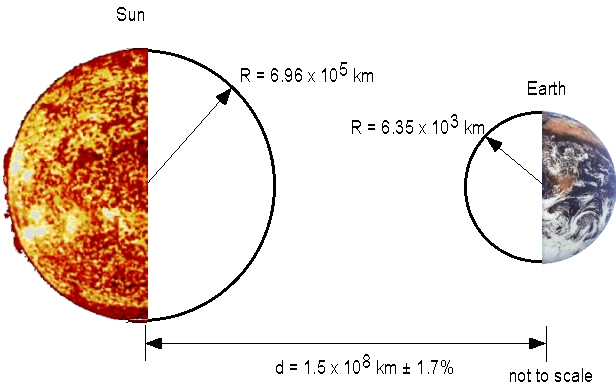
\includegraphics[width=0.6\textwidth]{figures/figure6_Sun_Earth.jpg}
\caption{Picture from \href{http://www.pveducation.org}{\textcolor{red}{www.pveducation.org}}}
\end{figure}
\end{frame}
%%%%%%%%%%%%%%%%%%%%%%%%%%%%%%%%%%%%%%%%%%%%%%%%%%%%%%%%%%%%%%%%%%%%%%%%%%%%%%%%%%%%%%%%%%%%%%%%%%%%%%%%%%%%%%%%




% slide # 9
%%%%%%%%%%%%%%%%%%%%%%%%%%%%%%%%%%%%%%%%%%%%%%%%%%%%%%%%%%%%%%%%%%%%%%%%%%%%%%%%%%%%%%%%%%%%%%%%%%%%%%%%%%%%%%%%
\begin{frame}

\begin{center}
    \textbf{\Large Distribution of power from solar spectrum}
\end{center}

\begin{columns}

\begin{column}{0.48\textwidth}
 \begin{center}
    \textbf{No high-energy filter}

  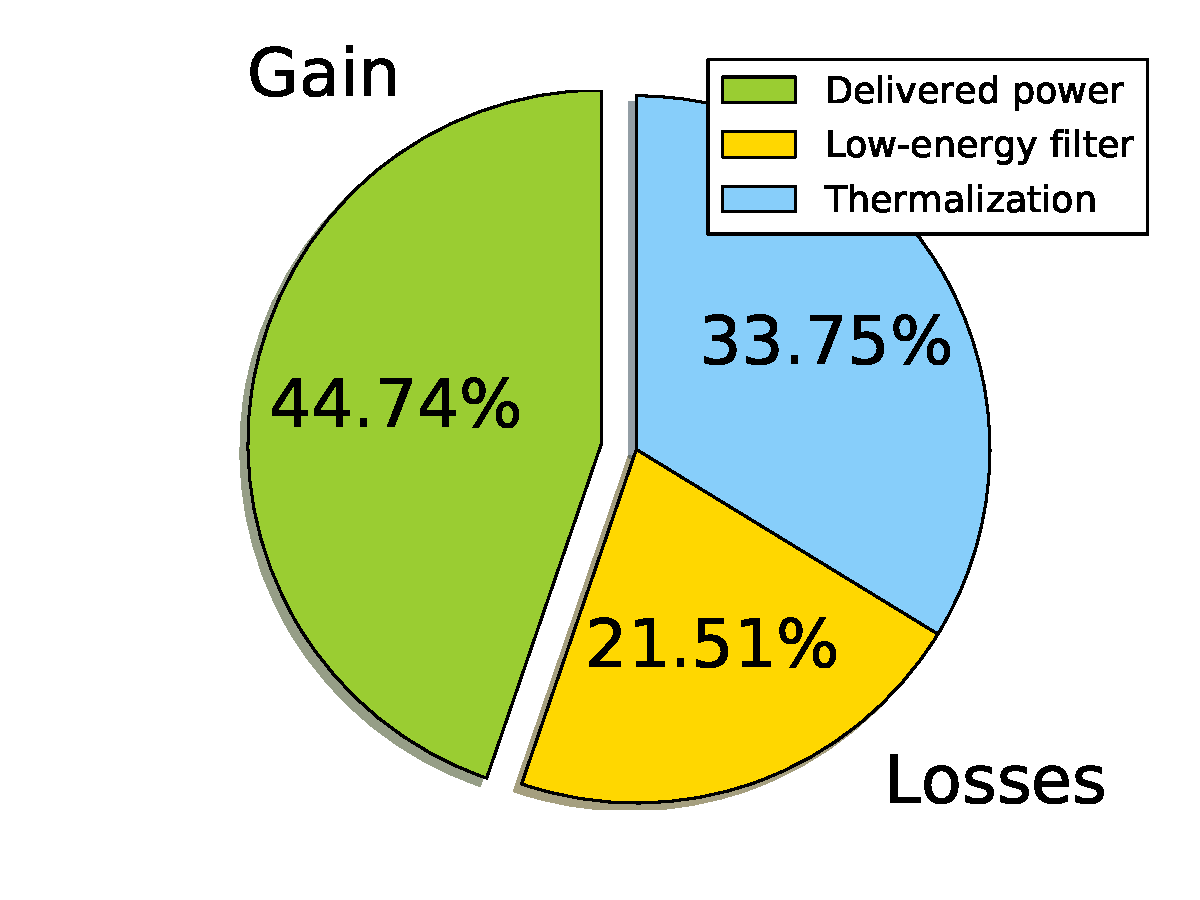
\includegraphics[width=1.0\textwidth]{figures/bar_chart/pie_cart1.pdf} 

  %\scriptsize
  \tiny
  \begin{tabular}{l||c||c}
    Power                &   \%    &  kW/m$^2$\\
    \hline
    \hline
    % Total power              & 100   & 1.458 \\
    Delivered (useful)   & 44.73   & 0.652 \\
    Thermalization       & 33.74   & 0.492 \\
    Low-energy filtered  & 21.51   & 0.314 \\
  \end{tabular}
 \end{center}
\end{column}

\begin{column}{0.48\textwidth}

 \begin{center}
    \textbf{With high-energy filter}

  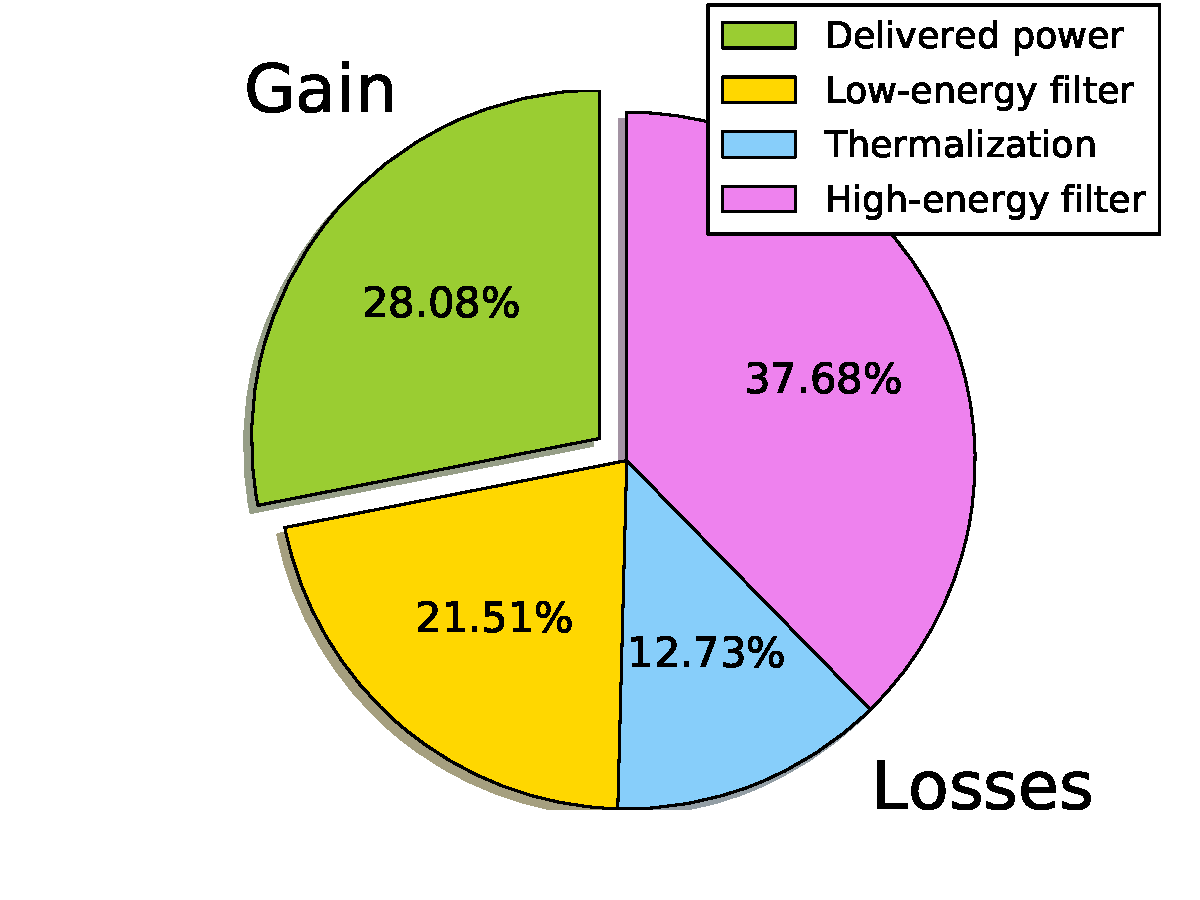
\includegraphics[width=1.0\textwidth]{figures/bar_chart/pie_cart2.pdf} 

  %\scriptsize
  \tiny
  \begin{tabular}{l||c||c}
    Power                &   \%    &  kW/m$^2$\\
    \hline
    \hline
    % Total power              & 100   & 1.458 \\
    Delivered (useful)   & 28.08   & 0.409 \\
    Thermalization       & 12.73   & 0.186 \\
    Low-energy filtered  & 21.51   & 0.314 \\
    High-energy filtered & 37.68   & 0.549 \\
  \end{tabular}

 \end{center}
\end{column}

\end{columns}

\end{frame}
%%%%%%%%%%%%%%%%%%%%%%%%%%%%%%%%%%%%%%%%%%%%%%%%%%%%%%%%%%%%%%%%%%%%%%%%%%%%%%%%%%%%%%%%%%%%%%%%%%%%%%%%%%%%%%%%




% Slide # 10
%%%%%%%%%%%%%%%%%%%%%%%%%%%%%%%%%%%%%%%%%%%%%%%%%%%%%%%%%%%%%%%%%%%%%%%%%%%%%%%%%%%%%%%%%%%%%%%%%%%%%%%%%%%%%%%%
\begin{frame}
\vspace{-0.2cm}
\begin{center}
    \textbf{\Large Distribution of power from solar spectrum}
\end{center}

\vspace{-0.6cm}

\begin{columns}

\begin{column}{0.45\textwidth}
 \begin{center}
    \textbf{No high-energy filter}

  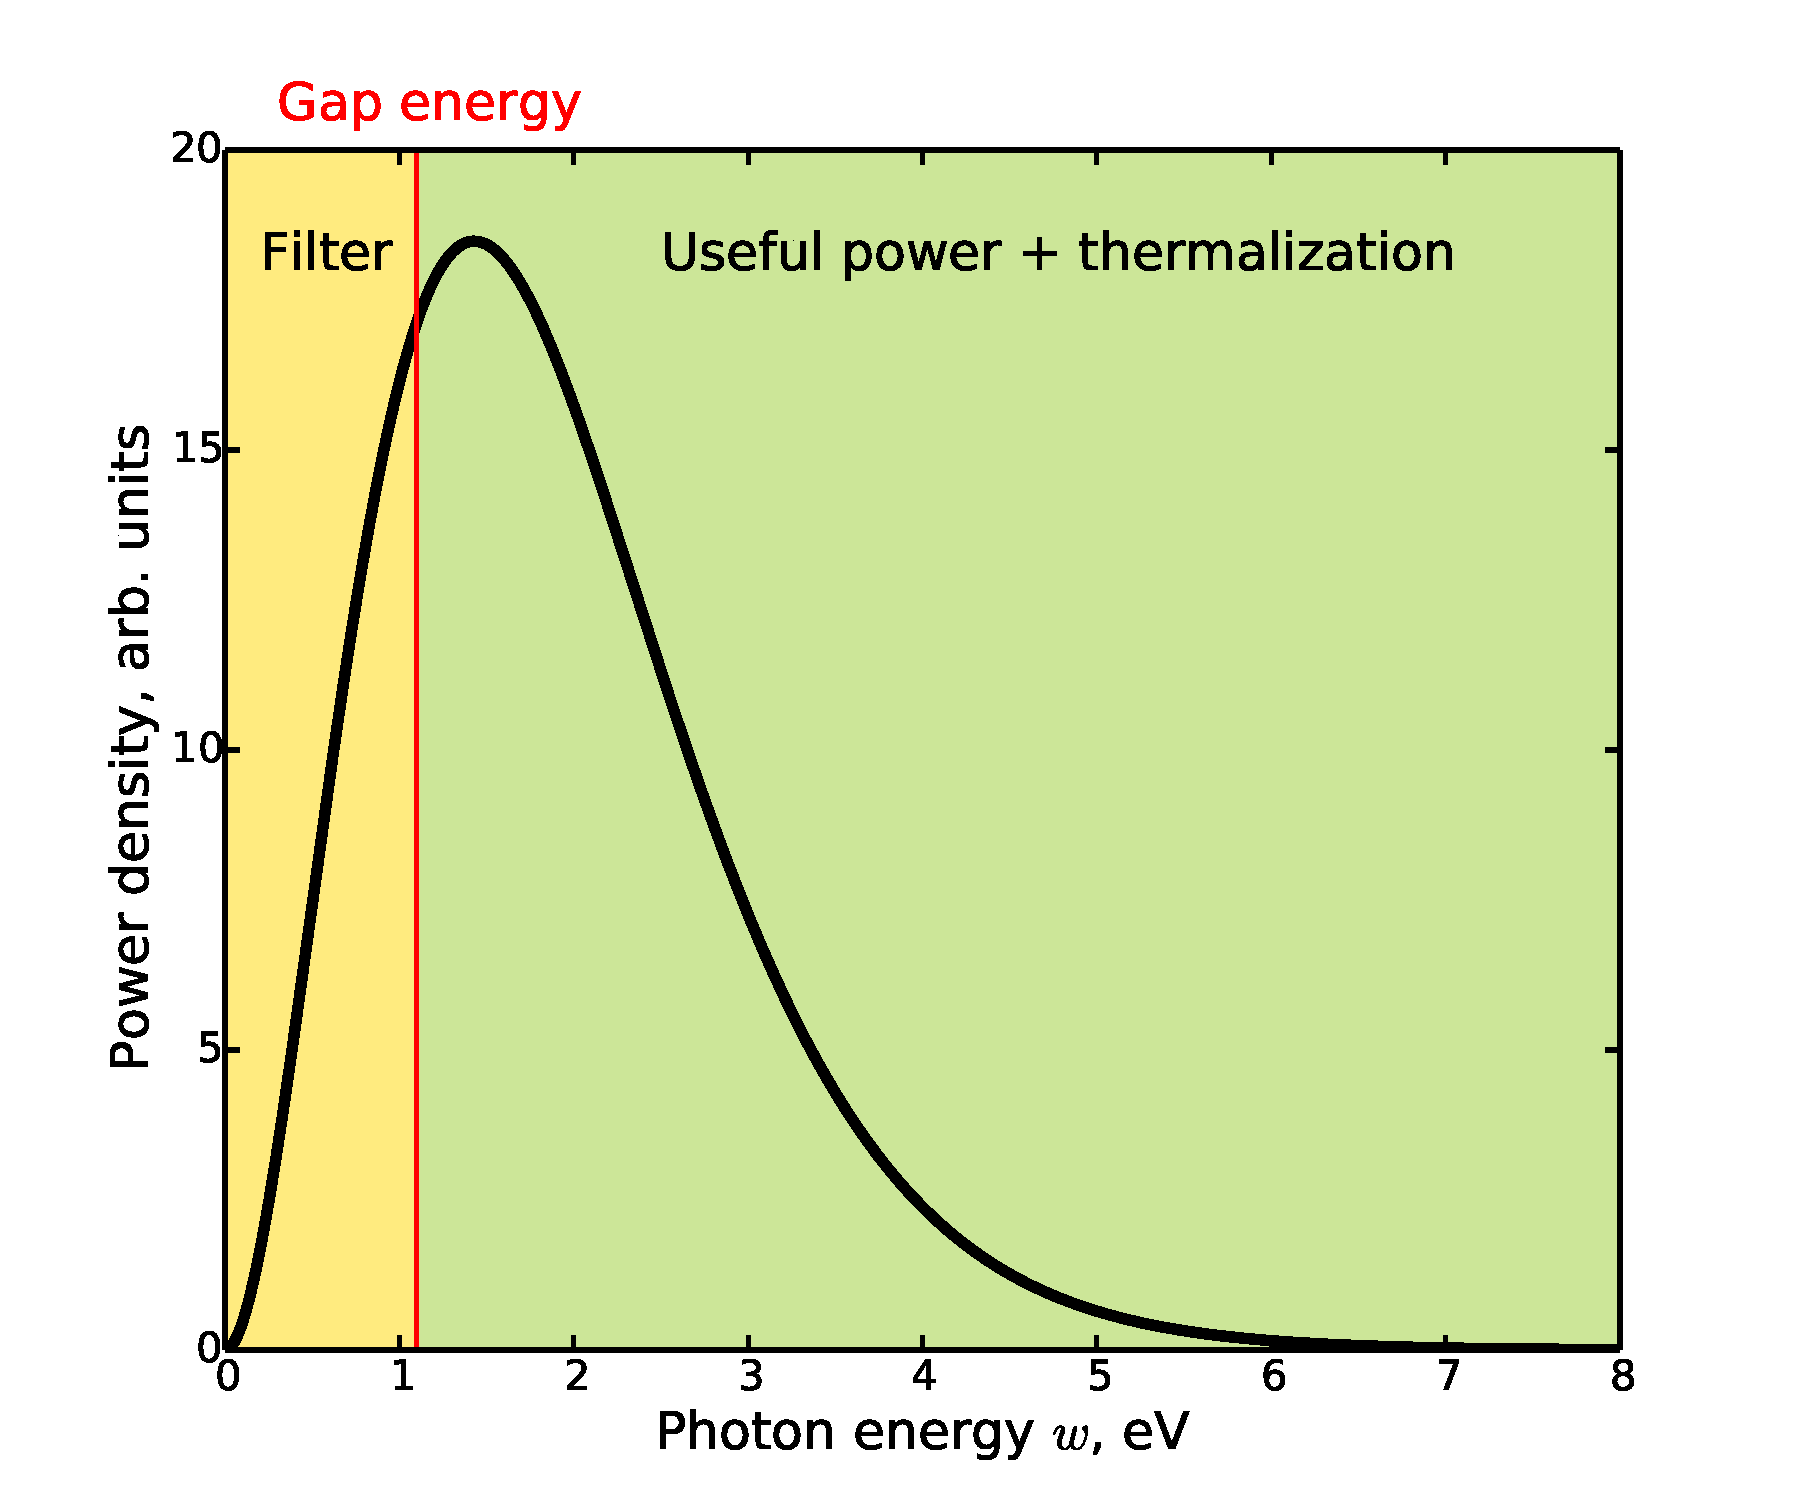
\includegraphics[width=1.0\textwidth]{figures/solar_spectrum/Planck-spectrum1.pdf} 
 \end{center}
\end{column}

\begin{column}{0.45\textwidth}

 \begin{center}
    \textbf{With high-energy filter}

  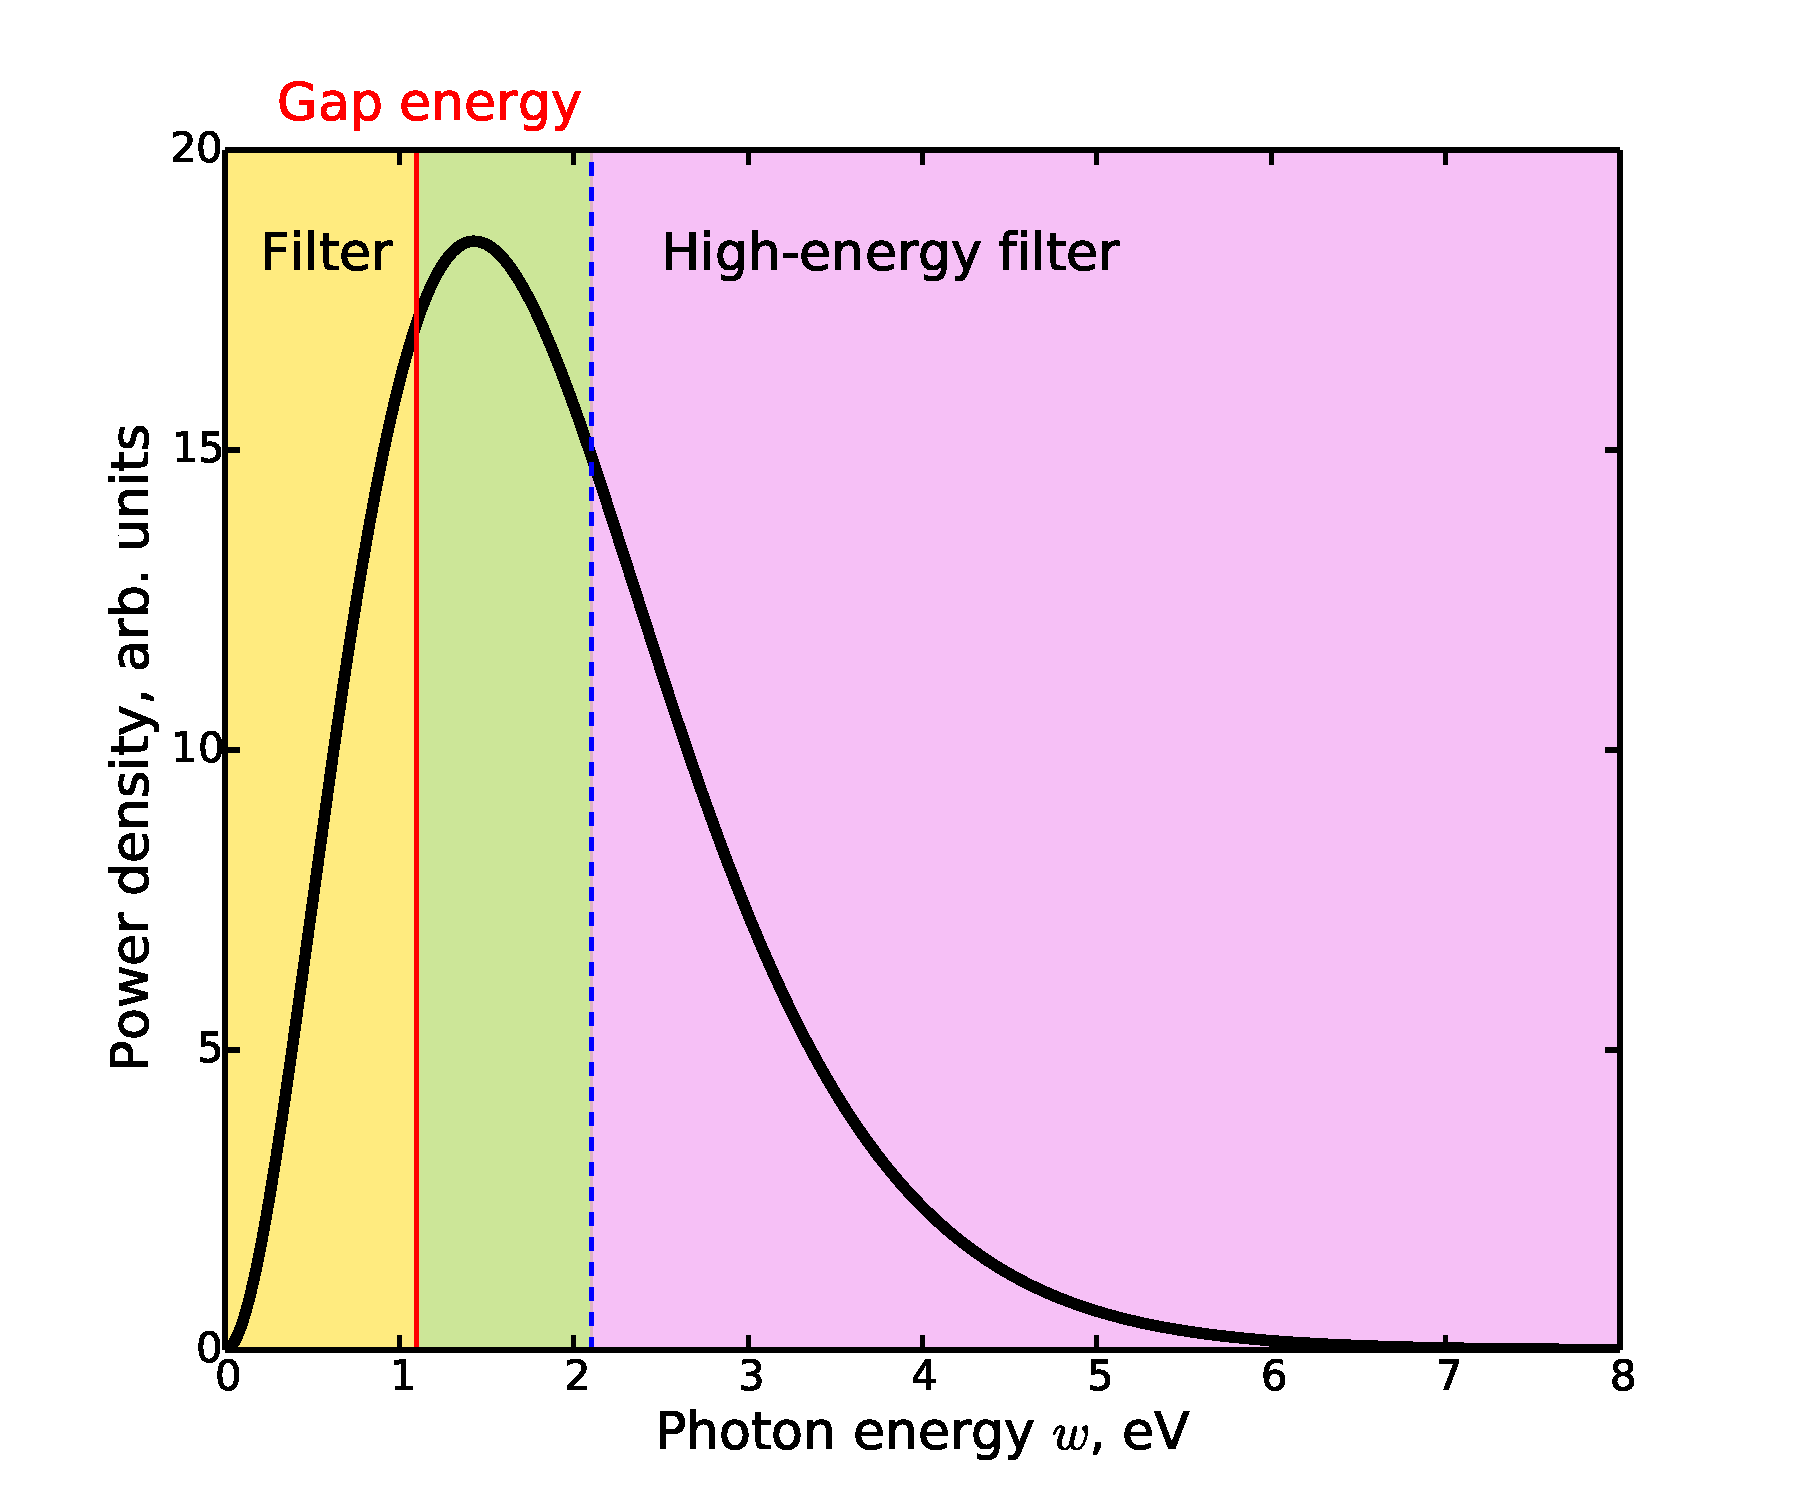
\includegraphics[width=1.0\textwidth]{figures/solar_spectrum/Planck-spectrum2.pdf} 

 \end{center}
\end{column}

\end{columns}

\vspace{-0.3cm}

 \begin{center}
 \textbf{Accumulated function}
 
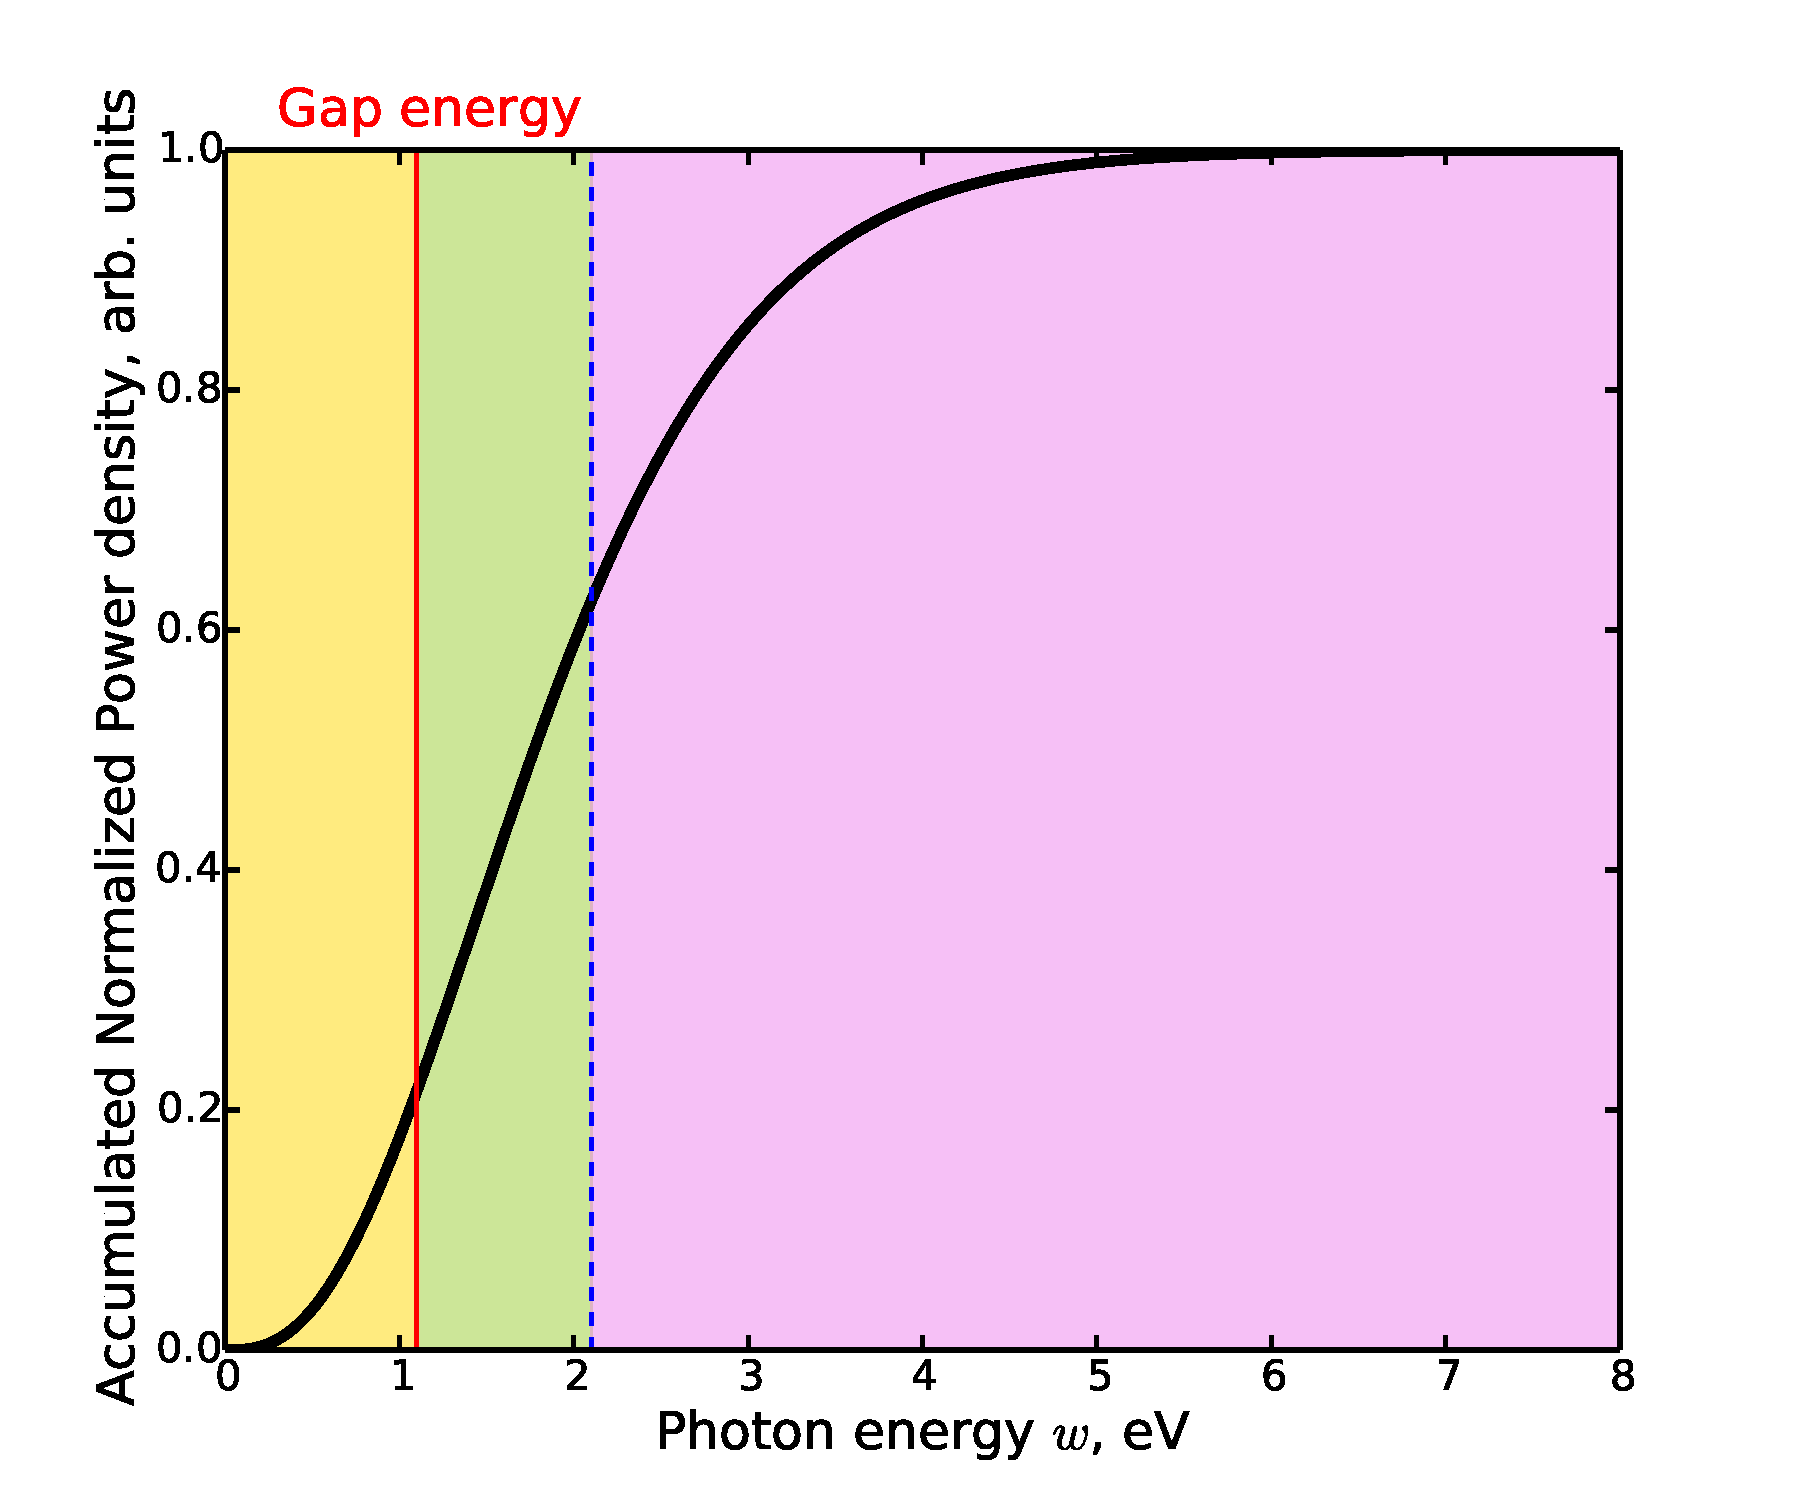
\includegraphics[width=0.45\textwidth]{figures/solar_spectrum/Accumulated_power.pdf}
 \end{center}
 
\end{frame}
%%%%%%%%%%%%%%%%%%%%%%%%%%%%%%%%%%%%%%%%%%%%%%%%%%%%%%%%%%%%%%%%%%%%%%%%%%%%%%%%%%%%%%%%%%%%%%%%%%%%%%%%%%%%%%%%




% Slide # 11
%%%%%%%%%%%%%%%%%%%%%%%%%%%%%%%%%%%%%%%%%%%%%%%%%%%%%%%%%%%%%%%%%%%%%%%%%%%%%%%%%%%%%%%%%%%%%%%%%%%%%%%%%%%%%%%%
\begin{frame}%

\begin{center}
 \textcolor{blue}{\textbf{Use of the high-energy part of solar spectrum}}
\end{center}

\begin{center}
\textbf{\textcolor{red}{Trupke}} \textit{\textcolor{red}{et al:}} \textbf{luminescence down-converter transforming high-energy photons to several photons of lower energies}
\end{center} 
 \vspace{-0.2cm}
 \begin{columns}

\begin{column}{0.45\textwidth}
 \begin{center}

  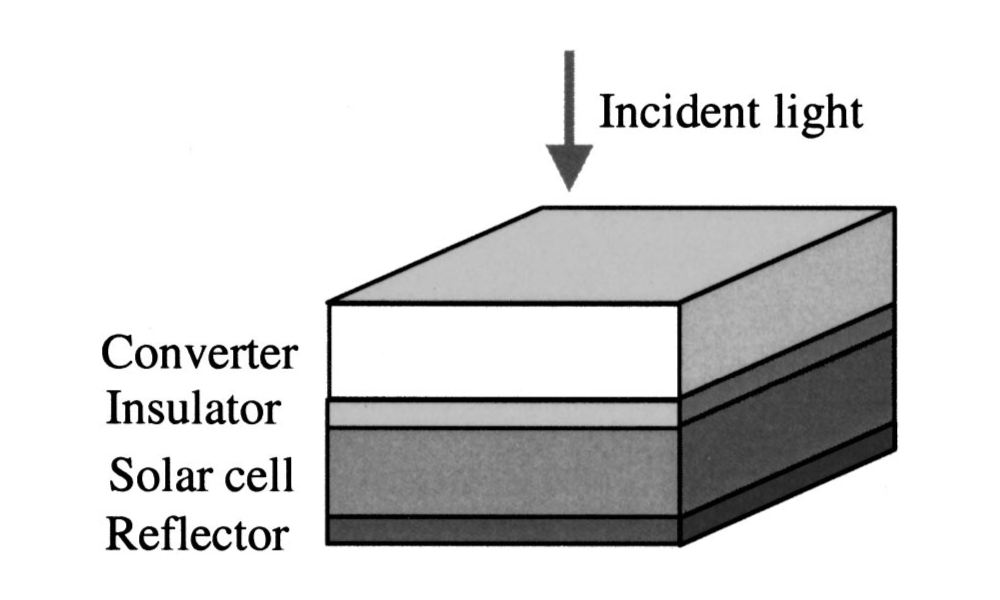
\includegraphics[width=0.9\textwidth]{figures/figure7_down-converter.jpeg} \\
\tiny \textbf{Schematic diagram of the down-conversion system}
\begin{itemize}
 \item \textcolor{red}{\textbf{Geometry 1:}}\\ \textbf{Converter}-Insulator-\textbf{Solar cell}-Reflector
 \item \textcolor{red}{\textbf{Geometry 2:}}\\ \textbf{Solar cell}-Insulator-\textbf{Converter}-Reflector
\end{itemize}

  
  \vspace{2cm}
  
  \end{center}
\end{column}

\begin{column}{0.45\textwidth}

 \begin{center}

  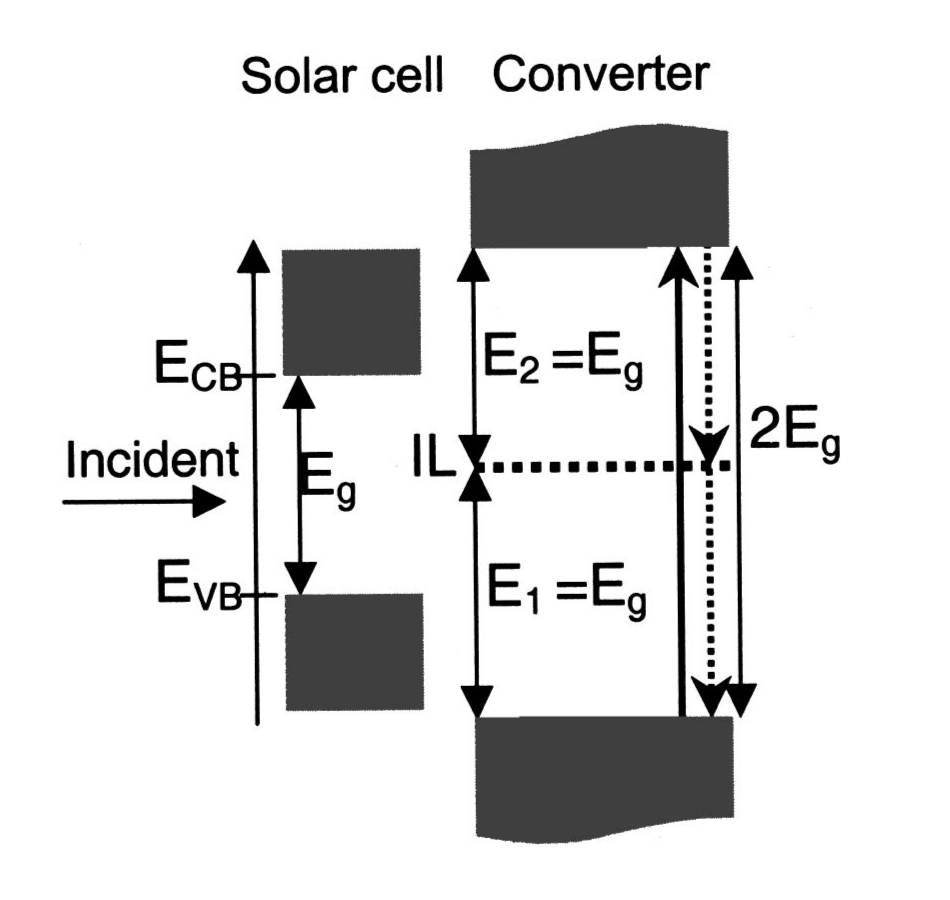
\includegraphics[width=0.9\textwidth]{figures/figure8_down-converter-scheme.jpeg} 
\vspace{-0.2cm}
\tiny\textbf{\underline{Three-level system:}}
\begin{enumerate}
 \item \textbf{Absorption} of high-energy photon
 \item \textbf{Excitation} of electron to the highest excited level.
 \item Two-step \textbf{recombination} of the electron to the lowest level via the intermediate impurity with \textcolor{red}{\textbf{emission of two lower energy photons}}.
\end{enumerate}

 \end{center}
\end{column}

\end{columns}

\vspace{0.1cm}

\tiny At low light intensities the major fraction of electron-hole pairs recombines via two intermediate transitions rather than by a band-to-band
transition from the conduction band to the valence band - Truple \textit{et al} J. Appl. Phys. \textbf{92}, 4117 (2002);
 
\end{frame}
%%%%%%%%%%%%%%%%%%%%%%%%%%%%%%%%%%%%%%%%%%%%%%%%%%%%%%%%%%%%%%%%%%%%%%%%%%%%%%%%%%%%%%%%%%%%%%%%%%%%%%%%%%%%%%%%


% End of file
\end{document}
